\part{ОПТИМИЗАЦИЯ}
    Метод Гаусса-Зейделя ($GZ_1$) сводит задачу поиска наименьшего значения функции нескольких переменных к многократному решению одномерных задач оптимизации, по сути это постепенное в многократном цикле сдвигание к результату.
    \setcounter{section}{0}
    \section{Алгоритм метода оптимизации $GZ_1$}
        \begin{center}
            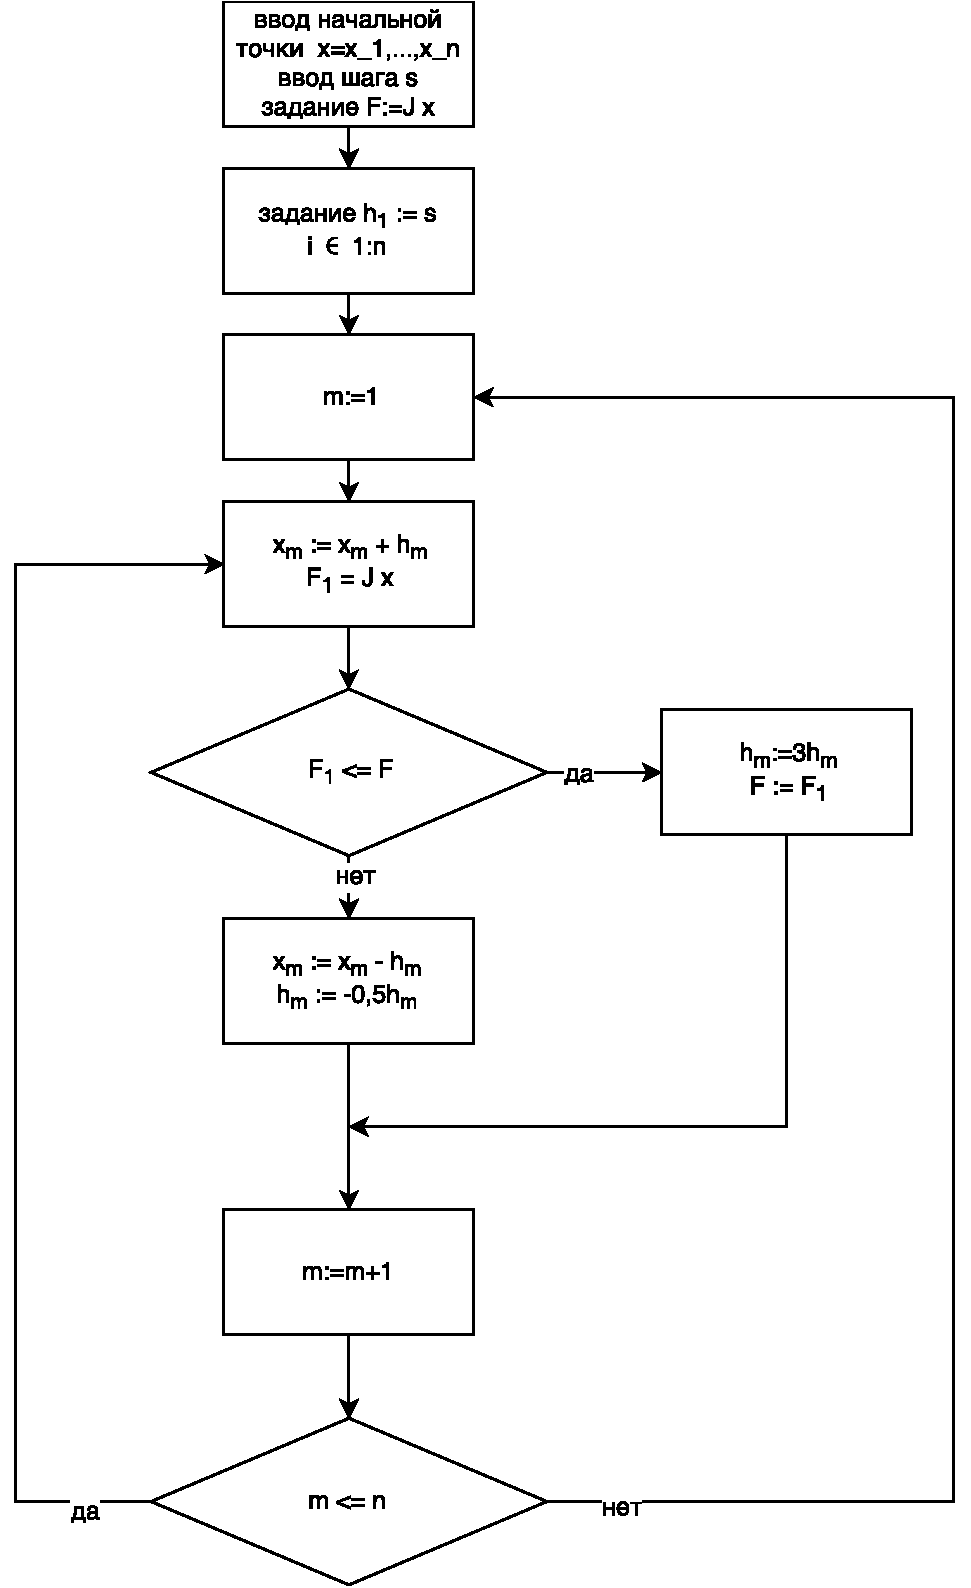
\includegraphics[scale=.6]{img/gz1-alg}
        \end{center}
        Выход из алгоритма осуществляется по достижении заданного числа вычислений $J$. В данном случае целесообразно отказаться от применения каких-либо внутренних критериев сходимости процесса оптимизации и обрывать его после заранее обусловленного числа шагов.

    \section{Проверка работоспособности}
        Проверка работоспособности функции была произведена на двух канонических функциях при различных начальных условиях. Для функции Розенброка значение функции стремилось всегда к $0$, а $x1, x2$ к 1. Для квадратичной функции все неизвестные стремились к $0$.

        \subsection{Функция Розенброка}
        %     \begin{center}
        %         \begin{tikzpicture}
        %             \begin{axis}[
        %                 width=16cm,
        %                 height=10cm,
        %                 samples=1,
        %                 minor tick num = 1,
        %                 grid = both
        %             ]

        %             \addplot[gr1] table {data/2points.dat};

        %             \end{axis}
        %         \end{tikzpicture}
        %     \end{center}

        \subsection{Квадратичная функция}
        %     \begin{center}
        %         \begin{tikzpicture}
        %             \begin{axis}[
        %                 width=16cm,
        %                 height=10cm,
        %                 samples=1,
        %                 minor tick num = 1,
        %                 grid = both
        %             ]

        %             \addplot[gr1] table {data/3points.dat};

        %             \end{axis}
        %         \end{tikzpicture}
        %     \end{center}
